\documentclass{beamer}
%\documentclass[handout]{beamer}

\usepackage{pgfpages} 

%\pgfpagesuselayout{4 on 1}[letterpaper,border shrink=5mm,landscape] 
%\pgfpagesuselayout{2 on 1}[letterpaper,border shrink=2mm]

\setbeameroption{show notes on second screen=left}
%\setbeameroption{show only notes}

\usetheme{default}

\mode<presentation> {
%  \usetheme{Warsaw}
  \usetheme{Frankfurt}
%  \usetheme{Boadilla}
%  \usetheme{Marburg}
}

\mode<handout>{\setbeamercolor{background canvas}{bg=black!5} %
    \pgfpagesuselayout{2 on 1}[letterpaper,border shrink=4mm] }

\title[CAC Intro] {A Introduction to\\ MPI}
\author{Brock Palen\\ \texttt{brockp@umich.edu}}

\begin{document}
  \setbeamercovered{transparent}  
  \begin{frame}
    \titlepage
  \end{frame}

%table of contents
  \begin{frame}{Outline}
    \tableofcontents
  \end{frame}
  
\section{Overview}
 \subsection {What is MPI?}

\begin{frame}{MPI}
 \begin{block}{MPI}
   \begin{itemize}
     \item MPI - Message Passing Interface
       \note[item]{\url{http://en.wikipedia.org/wiki/Message\_Passing\_Interface}}
       \note[item]{MPI Standard: \url{http://www.mpi-forum.org/}}
     \item C/C++/F77/F90 Bindings
       \note[item]{\texttt{man MPI\_Send} for prototypes}
     \item Distributed Memory Programming
     \item Series of Functions
   \end{itemize}
 \end{block}
   \begin{block}{Assumptions}
     \begin{itemize}
       \item All examples work on \texttt{nyx-login.engin.umich.edu}
       \item Used with OpenMPI built with the PGI Compilers
     \end{itemize}
   \end{block}
\end{frame}

 \subsection{Alternatives}
  \begin{frame}{MPI's Flow}
   \begin{center}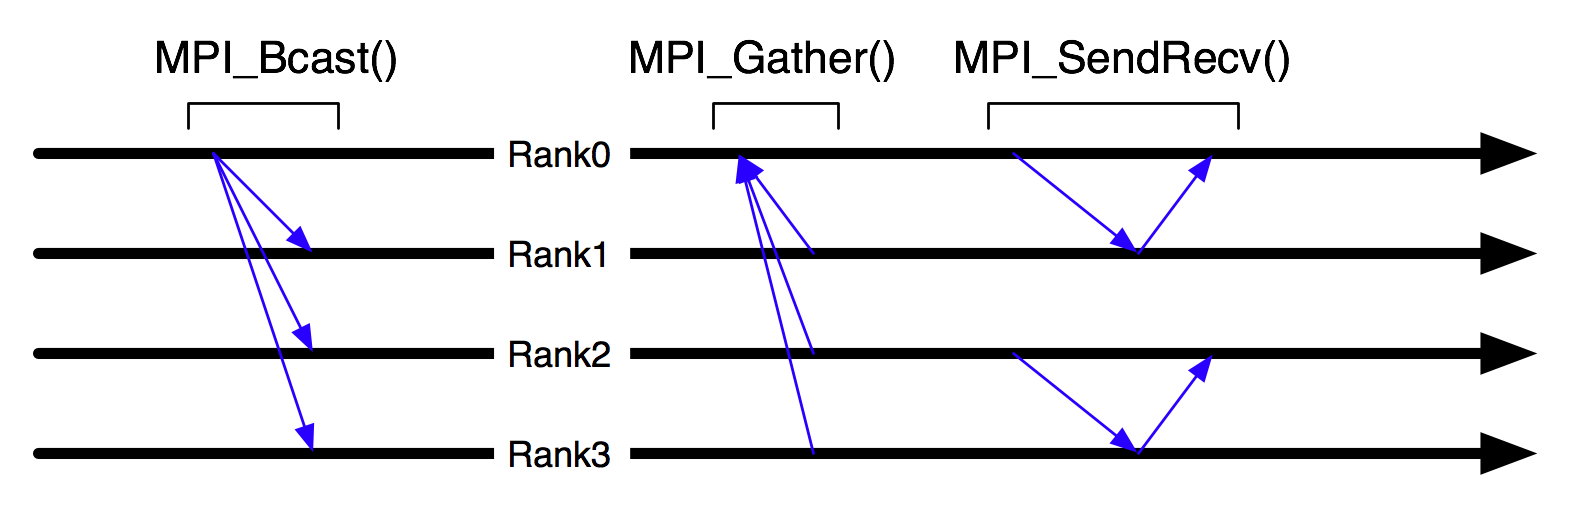
\includegraphics[height=1.5in]{mpi}\end{center}
    \note {MPI-All processes (normally one cpu per proccess but could be more) execute the same code. 
           These processes only know 'who they are' (their Rank). These ranks then have to explicitly 
           pass data.  This passing follows the form:
            \begin{enumerate}
              \item{Process 1 'Send to process 2'}
              \item{Process 2 'Recv from process 1'}
            \end{enumerate}
              \par Others options Colectives: \\ 
               \begin{itemize}
                \item {All process in a single Communicator,  'ALL DO THIS'}
               \end{itemize}
    } %note
  \end{frame}
  \begin{frame}{OpenMP}
   \begin{center}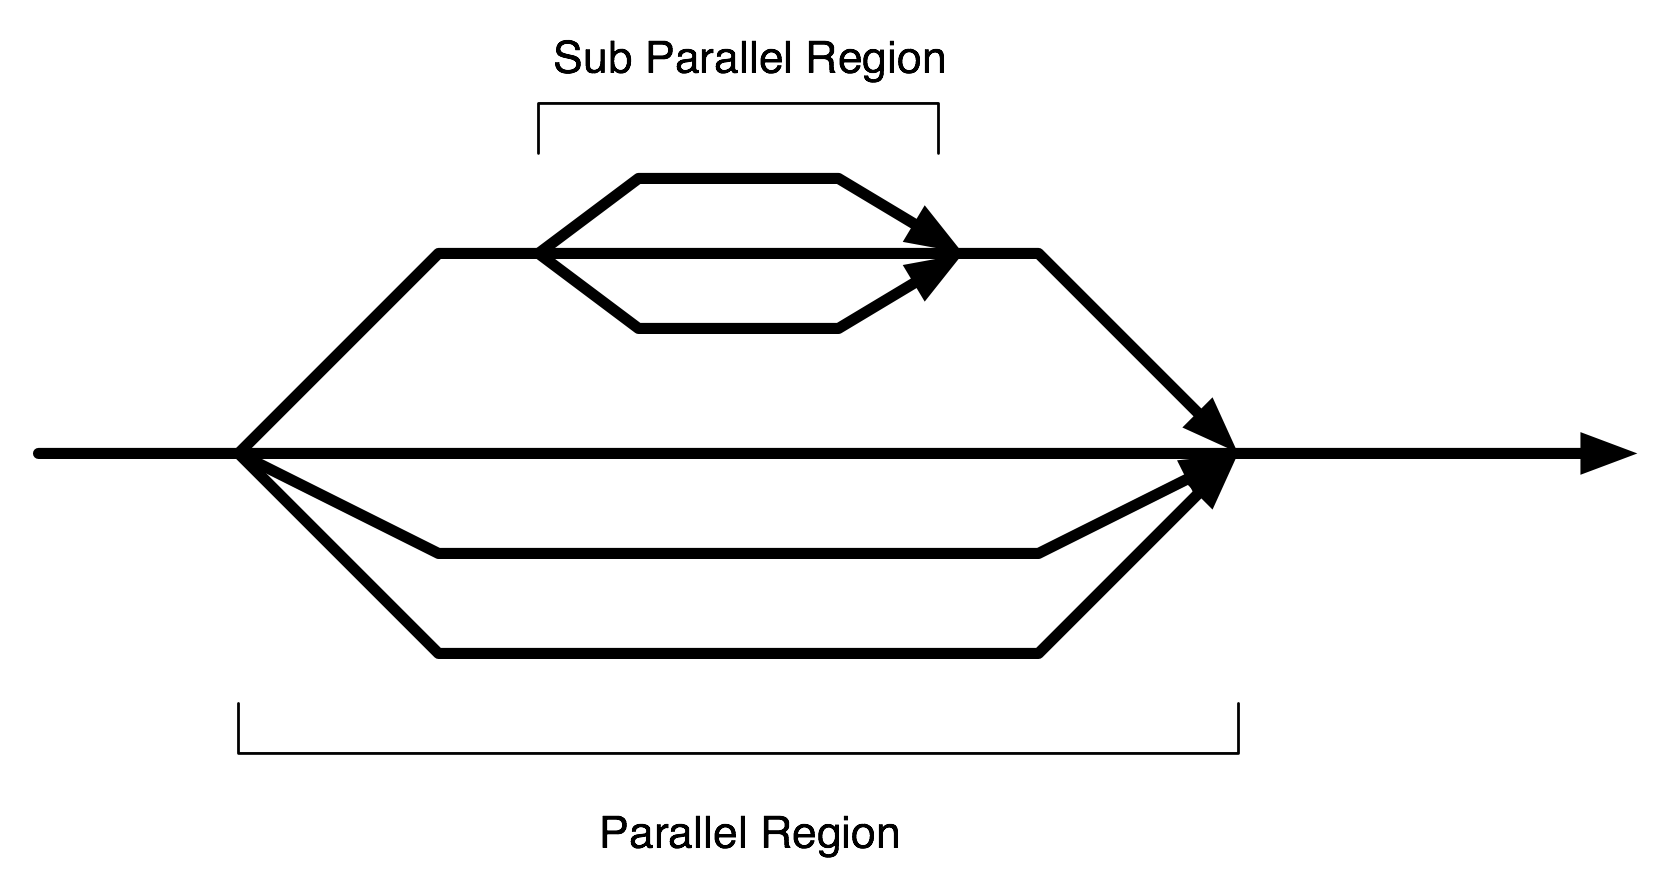
\includegraphics[height=2.5in]{openmp}\end{center}
   \note{OpenMP \url{http://www.openmpi.org} (Not to be confused with OpenMPI) is
         implimented in the compiler. Each compiler has its own issues with their 
         own implimentation of OpenMP but most users should find no problems with the basics.
         \begin{itemize}
           \item Anything that uses \texttt{OMP\_NUM\_THREADS} uses OpenMP
           \item PGI Compilers: \texttt{pgf90 -mp openmp.f90}
           \item Intel Compilers: \texttt{ifort -openmp openmp.f90}
         \end{itemize}
   }
  \end{frame}
  \begin{frame}{Other Options}
    \begin{block}{Other Options}
     \begin{itemize}
      \item<1->HPF-High Performance Fortran -- Use OpenMP/MPI
       \note[item]{HPF, \url{http://hpff.rice.edu/}}
      \item<2->pthreads -- Use OpenMP
       \note[item]{pthreads, \url{http://en.wikipedia.org/wiki/POSIX\_Threads}}
      \item<3->PVM -- Dead, Not installed, Use MPI
       \note[item]{PVM,\url{http://www.csm.ornl.gov/pvm/}}
      \item<4->CoArray
       \note[item]{CoArray, \url{http://www.co-array.org/}}
      \item<4-> Shmem -- Use \texttt{MPI\_Get()} and \texttt{MPI\_Put()}
       \note[item]{Shmem, \url{http://www.sgi.com/products/software/mpt/}}
     \end{itemize}
    \end{block}
  \end{frame}

  \section{Code}
   \subsection{Mechanics}
   \begin{frame}{MPI Mechanics}
    \begin{block}{Parts of an MPI Message}
     \begin{itemize}
     \item<1->{ Address of data, called a buffer}
     \item<1->{ MPI Datatype}
     \item<1->{ Count, or number of MPI datatypes to message}
     \item<2->{ Tag, Used to seperate messages from the same processor}
     \item<3->{ Communicator}
     \item<4->{ Rank of target}
     \end{itemize}
    \end{block}
    \note{
     MPI uses the buffer address, datatype and count to find how much raw data to send.
     For example, if MPI\_DOUBLE is 8 bytes, and count is 10, MPI 'knows' to send 80 bytes (10*8bytes) to the target process.  \\
     Note that \texttt{std::vector} is not a valid buffer for MPI! (or any STL class).  The STL does not make sure that all memory in continous. This breaks MPI, remember all buffers must be well defined. 

  } %end note
   \end{frame}
  \subsection{Utility Functions}
  \begin{frame}[fragile]
  \frametitle{MPI\_Init() MPI\_Finallize()}
   \begin{columns}[T]
    \begin{column}{5cm}
     \begin{block}{C}
      \begin{semiverbatim}
MPI\_Init(int  *argc,
          char ***argv)

MPI\_Finalize()
      \end{semiverbatim}
     \end{block}
    \end{column}
    \begin{column}{5cm}
     \begin{block}{Fortan}
      \begin{semiverbatim}
INTEGER IERROR
MPI\_INIT(IERROR)

MPI\_FINALIZE(IERROR)
      \end{semiverbatim}
     \end{block}
    \end{column}
   \end{columns}
   \begin{itemize}
     \item<2-> MPI\_Init() and MPI\_Finalize() should only be called once
     \item<3-> No other MPI calls are valid outside these functions
   \end{itemize}
\end{frame}

\begin{frame}
 \frametitle{Communicators and Tags}
  \begin{block}{Communicators}
   \begin{itemize}
     \item<1->Specifies a group of processors that can communicate together
     \item<2->\texttt{MPI\_COMM\_WORLD}
     \item<2->Created at startup includes all processes started by the launcher
   \end{itemize}
  \end{block}
  \begin{block}{Tags}
    \begin{itemize}
     \item<3->Adds distinct meaning to a message
     \item<4->Very Useful
    \end{itemize}
  \end{block}
\note{
 \begin{itemize}
  \item \textbf{Communicators}
  \item There can be more than one communicator
  \item They can be duplicated \texttt{MPI\_Comm\_dup()}
  \item They can be created \texttt{MPI\_Comm\_create()}
  \item They can have physical meaning \texttt{MPI\_Cart\_create()}
 \end{itemize}
 \begin{itemize}
  \item \textbf{Tags}
  \item \texttt{MPI\_ANY\_TAG} 
  \item \texttt{Information on tag available in \texttt{MPI\_Status}}
 \end{itemize}
} %note

\end{frame}

\begin{frame}[fragile]
 \frametitle{MPI\_DATATYPE}
  \begin{columns}[T]
   \begin{column}{5cm}
    \begin{block}{C}
     \begin{itemize}
      \item \texttt{MPI\_CHAR char}
      \item \texttt{MPI\_INT int}
      \item \texttt{MPI\_FLOAT float}
      \item \texttt{MPI\_DOUBLE double}
      \item \texttt{MPI\_Pack() struct}
     \end{itemize}
    \end{block}
   \end{column}
   \begin{column}{5cm}
    \begin{block}{Fortran}
     \begin{itemize}
      \item \texttt{MPI\_CHARACTER CHARACTER}
      \item \texttt{MPI\_INTEGER INTEGER}
      \item \texttt{MPI\_REAL REAL}
      \item \texttt{MPI\_DOUBLE\_PRECISION DOUBLE}
      \item \texttt{MPI\_COMPLEX COMPLEX}
      \item \texttt{MPI\_DOUBLE\_COMPLEX DBOUBLE\_COMPLEX}
     \end{itemize}
    \end{block}
   \end{column}
  \end{columns}
 \note{
 \begin{itemize}
  \item Unsigned and shorts also available
  \item Fortran can use \texttt{MPI\_REAL8 MPI\_INTEGER2} etc.
  \item C Structs must be 'packed' with \texttt{MPI\_Pack()}
  \item \url{http://www.lam-mpi.org/tutorials/one-step/datatypes.php}
 \end{itemize}
} %note
\end{frame}

\subsection{Point to Point}
\begin{frame}[fragile]
 \frametitle{MPI\_Send()}
   \begin{columns}[T]
    \begin{column}{5cm}
     \begin{block}{C}
      \begin{semiverbatim}
MPI\_Send( void  *buf,
           int count,
  MPI\_Datatype  type,
           int  dest,
           int   tag,
      MPI\_Comm   comm)
      \end{semiverbatim}
     \end{block}
    \end{column}
    \begin{column}{5cm}
     \begin{block}{Fortan}
      \begin{semiverbatim}
MPI\_SEND( <type>   BUF,
      INTEGER    COUNT,
 MPI\_Datatype     TYPE,
      INTEGER     DEST,
      INTEGER      TAG,
     MPI\_Comm     COMM,
      INTEGER    IERROR)
      \end{semiverbatim}
     \end{block}
    \end{column}
   \end{columns}
\note{
These are called 'blocking' sends. Note that MPI does not require that \texttt{MPI\_Send()} block, just that it not return untill \texttt{buf} is safe to use again. This can cause deadlocks to appear in code when scaled up. See the example included with this.
} %note
\end{frame}
\begin{frame}[fragile]
 \frametitle{MPI\_Recv()}
   \begin{columns}[T]
    \begin{column}{5cm}
     \begin{block}{C}
      \begin{semiverbatim}
MPI\_Recv( void   *buf,
           int  count,
  MPI\_Datatype   type,
           int source,
           int    tag,
      MPI\_Comm   comm,
    MPI\_Status  *status)
      \end{semiverbatim}
     \end{block}
    \end{column}
    \begin{column}{5cm}
     \begin{block}{Fortan}
      \begin{semiverbatim}
MPI\_RECV( <type>    BUF,
      INTEGER     COUNT,
 MPI\_Datatype      TYPE,
      INTEGER    SOURCE,
      INTEGER       TAG,
     MPI\_Comm      COMM,
      INTEGER    STATUS,
      INTEGER     IERROR)
      \end{semiverbatim}
     \end{block}
    \end{column}
   \end{columns}
\note{
In fortran STATUS must be: \texttt{integer status(MPI\_STATUS\_SIZE)}
The same issues apply here as MPI send. For every \texttt{MPI\_Send()} there must be a \texttt{MPI\_Recv()}. Most codes will put most of their communication time waiting for Recv's to actualy get their data. If there is no Send, Recv will wait forever.  See \texttt{MPI\_Irecv()} for non-blocking.
} %note
\end{frame}

\begin{frame}{First MPI Program}
\begin{block}{helloworld}
 \begin{enumerate}
  \item<1->\texttt{cp \~{}brockp/mpi-cac.tar \~{}}
  \item<1->\texttt{tar -xvf mpi-cac.tar}
  \item<1->\texttt{cd mpi-cac}
  \item<2-> C: \texttt{mpicc -o chello helloworld.c}
  \item<2-> F90: \texttt{mpif90 -o fhello helloworld.f90}
  \item<3-> mpirun -np 4 fhello
 \end{enumerate}
\end{block}
 \note{
  \texttt{mpi-cac.tar} includes a \texttt{Makefile} all examples can be built by running \texttt{make} or built one at a time, \texttt{make chello} will build the \texttt{helloworld.c} example.  While \texttt{make fapps} will build all fortran examples.  See \texttt{README} included for information.
 } %note
\end{frame}

\begin{frame}{Deadlocks}
 \begin{block}{Deadlock}
   \begin{itemize}
    \item Every \texttt{MPI\_Send()} must have a matching \texttt{MPI\_Recv()}
    \item A call that does not have a matching Send or Recv is deadlocked
    \item Calls do not return unless \texttt{buffer} is safe to reuse, \alert{not} that it was recved
    \item Some MPI libraries will let deadlocked code run untill messages reach a given size
   \end{itemize}
 \end{block}
 \begin{block}{cdeadlock}
  \begin{itemize}
   \item <2->\texttt{make cdeadlock no-cdeadlock}
   \item <2->\texttt{mpirun -np 4 cdeadlock}
   \item <2->\texttt{mpirun -np 4 no-cdeadlock}
  \end{itemize}
 \end{block}
 \note{
    This example will demonstrate the effects of deadlock, and eager messages. \\
    cdeadlock and no-cdeadlock is the same code, the change is in the size of \texttt{buffer} when buffer falls below some value eager messaging takes place. In this case the MPI library says the message is small enough, lets allocate memory copy the buffer to it and return right away, so the buffer is now safe to reuse allowing the code to continue.  In the cdeadlock/fdeadlock case these buffers are to large and MPI
 will not copy the code will block at \texttt{MPI\_Send()}  for forever.
} %note
\end{frame}

\begin{frame}{Deadlock Example}
   \begin{center}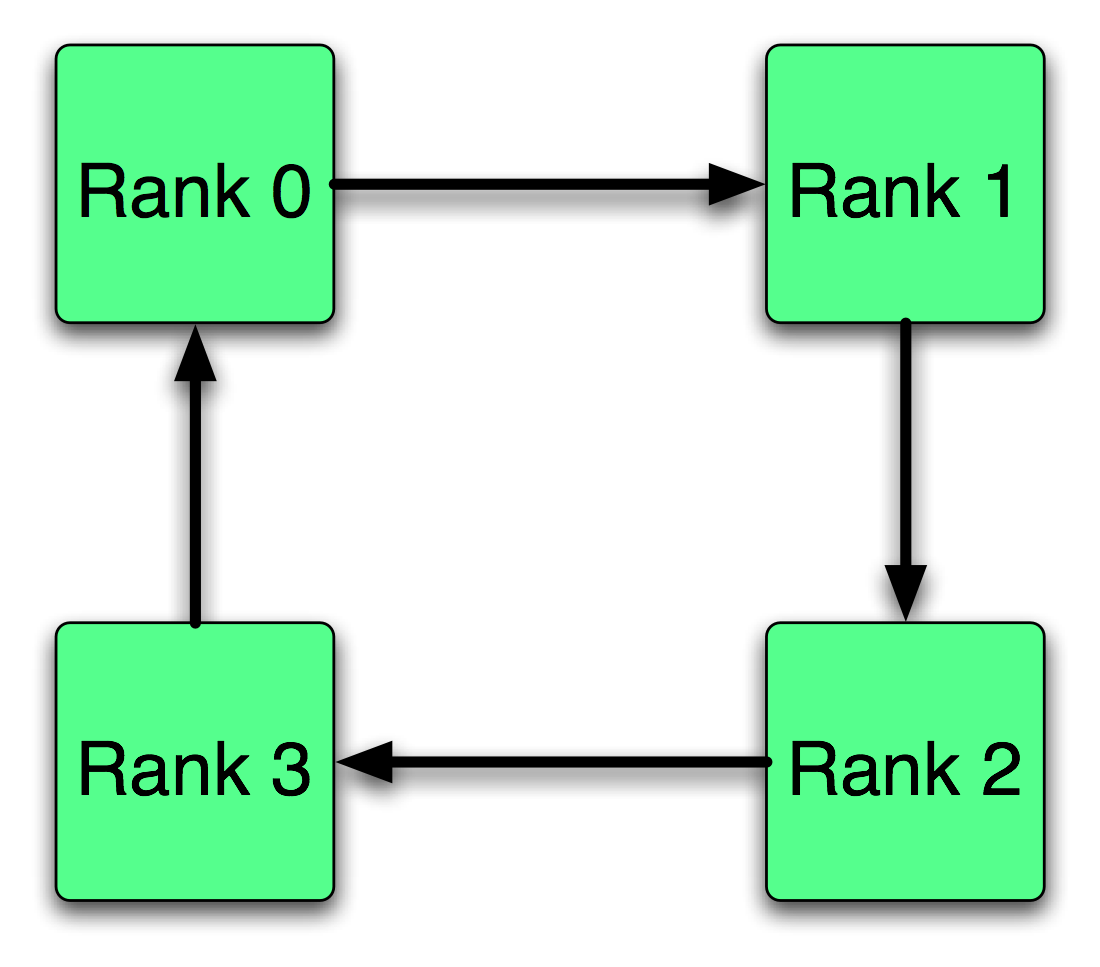
\includegraphics[height=3.0in]{deadlock}\end{center}
   \note{
    \begin{itemize}
      \item Each process does a \texttt{MPI\_Send()} to rank+1
      \item Each process then calls \texttt{MPI\_Recv()} from rank-1
      \item \texttt{make cdeadlock} or \texttt{make fdeadlock}
      \item \texttt{mpirun -np 4 cdeadlock}
      \item \texttt{make no-cdeadlock} or \texttt{make no-fdeadlock}
    \end{itemize}
} %notes
\end{frame} 
\end{document}
